\documentclass[conference]{IEEEtran}
\IEEEoverridecommandlockouts

\usepackage{cite}
\usepackage{amsmath,amssymb,amsfonts}
\usepackage{algorithmic}
\usepackage{graphicx}
\usepackage{textcomp}
\usepackage{xcolor}
\usepackage{hyperref}
\usepackage{booktabs}
\usepackage{multirow}
\usepackage{tikz}
\usetikzlibrary{positioning, arrows.meta, shapes.geometric, fit, calc, backgrounds}
\usepackage{pgfplots}
\pgfplotsset{compat=1.18}
\usepackage{bm}
\usepackage{siunitx}

\begin{document}

\title{Behavior-Aware Multi-Object Tracking via Interacting Multiple Models with Social Force Augmentation in CARLA}

\author{\IEEEauthorblockN{Rahul Ayanampudi}
\IEEEauthorblockA{\textit{AeroAstro Department} \\
\textit{Stanford University}\\
Palo Alto, United States \\
rayanam@stanford.edu}
\and
\IEEEauthorblockN{Aditya Kothari}
\IEEEauthorblockA{\textit{AeroAstro Department} \\
\textit{Stanford University}\\
Palo Alto, United States \\
kothari1@stanford.edu}
\and
\IEEEauthorblockN{Yash Rampuria}
\IEEEauthorblockA{\textit{AeroAstro Department} \\
\textit{Stanford University}\\
Palo Alto, United States \\
yashr@stanford.edu}
}

\maketitle

% ======================================================================
%  ABSTRACT
% ======================================================================
\begin{abstract}
Accurate state estimation of pedestrians is essential for safe autonomous driving in urban environments. Standard multi-object tracking pipelines typically rely on constant-velocity Kalman filters operating in image space, which fail to capture the non-linear, socially-influenced dynamics of pedestrian motion. We present a behavior-aware tracking framework that couples an Interacting Multiple Model (IMM) filter---blending Constant Velocity, Coordinated Turn, and Constant Deceleration models---with an exponential social force term injected directly into the filter prediction step. The filter operates entirely in three-dimensional world-frame coordinates obtained via RGB-D depth unprojection and is integrated into a DeepSORT data-association pipeline with a tuneable appearance-versus-motion cost parameter $\lambda$. We evaluate five tracker configurations against CARLA simulator ground truth across scenarios with one to five pedestrians over five randomized trials, measuring root-mean-square position error (RMSE) and identity switches (IDSW). Our results demonstrate that the behavior-aware IMM filter with balanced appearance--motion association ($\lambda{=}0.5$) achieves the lowest RMSE ($0.50\,\text{m}$ at 5~pedestrians) and fewest identity switches ($9.8$), reducing RMSE by $55\%$ and IDSW by $68\%$ compared to the motion-only vanilla Kalman filter baseline ($1.10\,\text{m}$, $30.2$ IDSW).
\end{abstract}

\begin{IEEEkeywords}
Multi-Object Tracking, State Estimation, Extended Kalman Filter, Interacting Multiple Model, Social Force Model, DeepSORT, CARLA Simulator
\end{IEEEkeywords}

% ======================================================================
%  1. INTRODUCTION
% ======================================================================
\section{Introduction}
\label{sec:intro}

Reliable perception of dynamic agents is a cornerstone of safety for autonomous vehicles operating in dense urban environments. Navigating alongside pedestrians requires not only detecting objects but accurately estimating their kinematic states and anticipating future behavior. A tracking system that treats each pedestrian as an isolated, inertia-driven particle---as standard constant-velocity Kalman filters do---cannot model social interactions such as collision avoidance, yielding, or group formation, leading to poor trajectory prediction and elevated identity-switch rates under occlusion~\cite{lefevre2014survey}.

This paper addresses these shortcomings through three contributions:
\begin{enumerate}
    \item A \textbf{behavior-aware Interacting Multiple Model (IMM)} filter that blends three kinematic hypotheses---constant velocity, coordinated turn, and constant deceleration---with a social force prediction term, operating entirely in 3-D world-frame coordinates.
    \item A \textbf{configurable data-association framework} built on DeepSORT~\cite{wojke2017simple} that blends Mahalanobis-distance gating from the IMM with appearance features via a tuneable parameter~$\lambda$, enabling systematic comparison of motion-only, appearance-only, and hybrid association strategies.
    \item A \textbf{controlled experiment pipeline} within the CARLA simulator~\cite{dosovitskiy2017carla} that sweeps pedestrian density from one to five agents across five tracker configurations, producing ground-truth-validated RMSE and IDSW metrics.
\end{enumerate}

The remainder of this paper is organized as follows. Section~\ref{sec:related} reviews related work on pedestrian tracking, behavior-aware filtering, and the IMM framework. Section~\ref{sec:method} details the system architecture, state-space formulation, dynamics models, social force augmentation, EKF measurement update, IMM mechanics, coordinate transformations, and data association. Section~\ref{sec:experiments} describes the CARLA experimental setup. Section~\ref{sec:results} presents quantitative and qualitative results. Section~\ref{sec:limitations} discusses limitations and future work, and Section~\ref{sec:conclusion} concludes.

% ======================================================================
%  2. RELATED WORK
% ======================================================================
\section{Related Work}
\label{sec:related}

\subsection{Multi-Object Tracking}
Modern multi-object tracking (MOT) follows a tracking-by-detection paradigm. Classical filtering remains the standard; the Kalman filter~\cite{kalman1960} and its non-linear variants (EKF, UKF) are widely used to recursively estimate object states~\cite{barshalom2001estimation, welch1995introduction}. However, tracking multiple agents introduces the data-association problem. While traditional approaches like the Joint Probabilistic Data Association (JPDA) filter offer theoretical rigor~\cite{barshalom1995multitarget}, modern tracking-by-detection methods have dominated recent benchmarks. SORT~\cite{bewley2016simple} pairs a constant-velocity Kalman filter with Hungarian assignment on IoU cost, achieving real-time performance but suffering from identity switches under occlusion. DeepSORT~\cite{wojke2017simple} augments SORT with a deep appearance descriptor and cascade matching, substantially reducing identity switches. ByteTrack~\cite{zhang2022bytetrack} recovers low-confidence detections via a second association stage. All of these methods operate in image space with linear motion models, limiting their ability to capture 3-D pedestrian dynamics.

\subsection{Behavior-Aware Prediction}
Helbing and Moln\'{a}r's Social Force Model (SFM)~\cite{helbing1995social} represents pedestrians as particles governed by attractive goal forces and repulsive social forces from neighbors. While recent deep-learning methods such as Social LSTM~\cite{alahi2016social} and Trajectron++~\cite{salzmann2020trajectron} learn complex interaction patterns from data, the SFM remains attractive for filter-based pipelines because it provides an analytically differentiable control input that can be injected directly into the EKF prediction step without retraining.

\subsection{Interacting Multiple Model Filters}
The IMM algorithm~\cite{blom1988imm, blackman1999design} maintains a bank of Kalman (or extended Kalman) filters, each embodying a different motion hypothesis, and blends their outputs via Bayesian model-probability weighting. Li and Jilkov~\cite{li2005survey} survey IMM variants for maneuvering target tracking, and Mazor et al.~\cite{mazor1998imm} demonstrate IMM superiority over single-model filters when targets switch between kinematic regimes. Our contribution extends the IMM framework by (i)~operating in 3-D world coordinates rather than 2-D image space, (ii)~incorporating social forces as a behavior-aware prediction input, and (iii)~embedding the filter within a DeepSORT association pipeline with a tuneable appearance--motion trade-off.

% ======================================================================
%  3. METHODOLOGY
% ======================================================================
\section{Methodology}
\label{sec:method}

% ------------------------------------------------------------------
%  3.1 System Architecture
% ------------------------------------------------------------------
\subsection{System Architecture}
\label{sec:pipeline}

Figure~\ref{fig:pipeline} illustrates the end-to-end pipeline. Raw RGB and depth frames from a forward-facing camera are processed offline. YOLOv9~\cite{wang2020yolo} produces 2-D bounding-box detections filtered to the \texttt{person} class; each detection is cropped and fed through an OSNet~\cite{zhou2019osnet} re-identification network to extract a 512-D appearance feature. The bounding-box center is back-projected to 3-D using the depth image and known camera intrinsics. These 3-D world-frame detections, along with appearance features, enter the DeepSORT tracker, which performs cascade matching and track management using either the behavior-aware IMM filter or a vanilla constant-velocity Kalman filter, depending on the experimental configuration.

\begin{figure*}[!t]
\centering
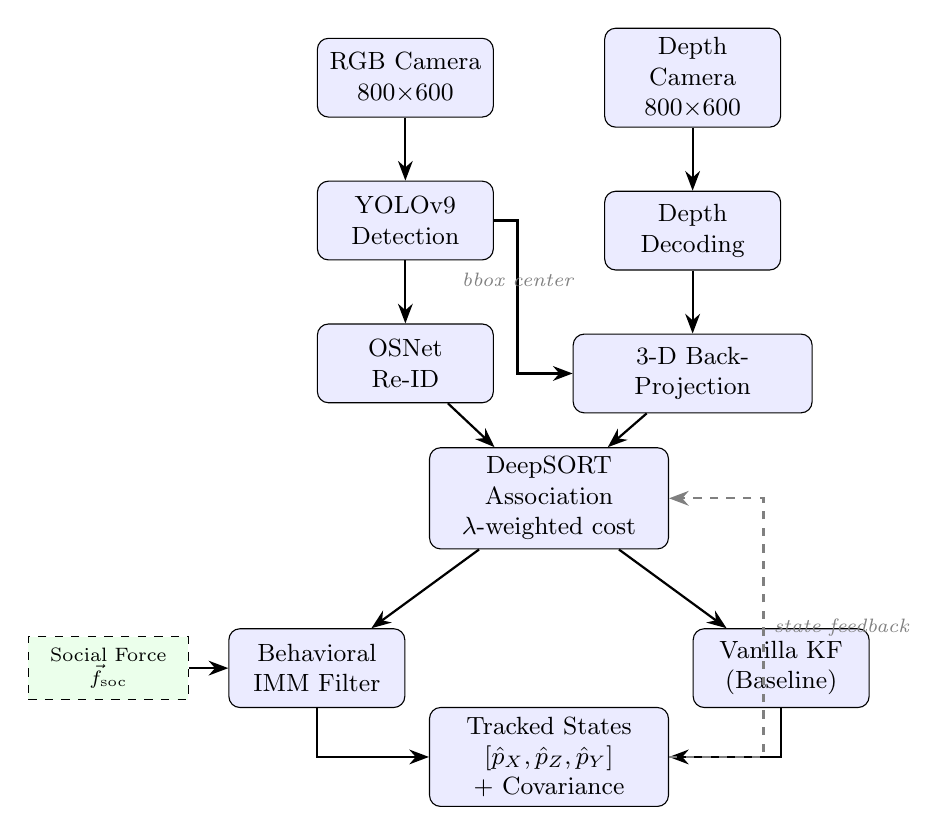
\begin{tikzpicture}[
    node distance=0.8cm and 1.2cm,
    block/.style={rectangle, draw, rounded corners, fill=blue!8,
                  minimum height=1.0cm, minimum width=2.0cm,
                  text width=2.0cm, align=center, font=\small},
    wideblock/.style={rectangle, draw, rounded corners, fill=blue!8,
                  minimum height=1.0cm, minimum width=2.8cm,
                  text width=2.8cm, align=center, font=\small},
    data/.style={rectangle, draw, dashed, fill=green!8,
                 minimum height=0.8cm, minimum width=1.8cm,
                 text width=1.8cm, align=center, font=\scriptsize},
    arr/.style={-{Stealth[length=2.5mm]}, thick},
    note/.style={font=\scriptsize\itshape, text=gray},
]

% Row 1: Sensors
\node[block] (rgb) {RGB Camera\\$800{\times}600$};
\node[block, right=1.4cm of rgb] (depth) {Depth Camera\\$800{\times}600$};

% Row 2: Detection / Depth
\node[block, below=0.8cm of rgb] (yolo) {YOLOv9\\Detection};
\node[block, below=0.8cm of depth] (depthproc) {Depth\\Decoding};

% Row 2.5: ReID + Unprojection
\node[block, below=0.8cm of yolo] (reid) {OSNet\\Re-ID};
\node[wideblock, below=0.8cm of depthproc] (unproj) {3-D Back-\\Projection};

% Row 3: Association
\node[wideblock, below=1.0cm of $(reid)!0.5!(unproj)$] (assoc) {DeepSORT\\Association\\$\lambda$-weighted cost};

% Row 4: Filter
\node[block, below left=1.0cm and 0.3cm of assoc] (imm) {Behavioral\\IMM Filter};
\node[block, below right=1.0cm and 0.3cm of assoc] (kf) {Vanilla KF\\(Baseline)};

% Row 4.5: Social force
\node[data, left=0.5cm of imm] (sf) {Social Force\\$\vec{f}_{\mathrm{soc}}$};

% Row 5: Output
\node[wideblock, below=1.2cm of assoc, yshift=-0.8cm] (output) {Tracked States\\$[\hat{p}_X, \hat{p}_Z, \hat{p}_Y]$\\$+$ Covariance};

% Arrows
\draw[arr] (rgb) -- (yolo);
\draw[arr] (depth) -- (depthproc);
\draw[arr] (yolo) -- (reid);
\draw[arr] (depthproc) -- (unproj);
\draw[arr] (reid) -- (assoc);
\draw[arr] (unproj) -- (assoc);
\draw[arr] (yolo.east) -- ++(0.3,0) |- (unproj.west) node[note, pos=0.25, above] {bbox center};
\draw[arr] (assoc) -- (imm);
\draw[arr] (assoc) -- (kf);
\draw[arr] (sf) -- (imm);
\draw[arr] (imm) |- (output);
\draw[arr] (kf) |- (output);

% Feedback arrow
\draw[arr, dashed, gray] (output.east) -- ++(1.2,0) |- (assoc.east)
    node[note, pos=0.25, right] {state feedback};

\end{tikzpicture}
\caption{End-to-end tracking pipeline. RGB frames are processed by YOLOv9 for detection and OSNet for re-identification. Depth frames provide 3-D back-projection of detection centers. The DeepSORT association layer blends appearance and Mahalanobis motion costs via $\lambda$. Matched detections update either the behavioral IMM filter (with social force input) or the vanilla KF baseline. Estimated world-frame states and covariances feed back into the next association step.}
\label{fig:pipeline}
\end{figure*}

% ------------------------------------------------------------------
%  3.2 State Space Formulation
% ------------------------------------------------------------------
\subsection{State Space Formulation}
\label{sec:state}

Each pedestrian is tracked in 3-D camera-frame coordinates. The per-model state vector is seven-dimensional:
\begin{equation}
\label{eq:state}
\mathbf{x} = \begin{bmatrix} p_X & p_Z & v & \phi & \omega & p_Y & v_Y \end{bmatrix}^\top
\end{equation}
where $p_X$ is the camera-right position (metres), $p_Z$ is the camera-forward position (depth, metres), $v$ is the horizontal speed in the $XZ$ plane, $\phi$ is the heading angle (radians), $\omega$ is the turn rate (rad/frame), $p_Y$ is the camera-down position (metres), and $v_Y$ is the vertical velocity (m/frame). Operating in 3-D world-frame rather than 2-D image space avoids the perspective distortion inherent in pixel-based tracking and enables the social force model to operate on metrically meaningful distances.

The full IMM state is packed into a 24-dimensional vector:
\begin{equation}
\label{eq:packed}
\mathbf{x}_{\text{IMM}} = \begin{bmatrix} \mathbf{x}_{\text{CV}}^\top & \mathbf{x}_{\text{CT}}^\top & \mathbf{x}_{\text{CA}}^\top & \mu_{\text{CV}} & \mu_{\text{CT}} & \mu_{\text{CA}} \end{bmatrix}^\top
\end{equation}
where $\mathbf{x}_{\text{CV}}, \mathbf{x}_{\text{CT}}, \mathbf{x}_{\text{CA}} \in \mathbb{R}^7$ are the per-model states and $\bm{\mu} = [\mu_{\text{CV}}, \mu_{\text{CT}}, \mu_{\text{CA}}]^\top$ are the mode probabilities summing to one. The associated covariance is block-diagonal in the $21{\times}21$ model-state partition, with the mode-probability entries stored separately.

% ------------------------------------------------------------------
%  3.3 Dynamics Models
% ------------------------------------------------------------------
\subsection{Dynamics Models}
\label{sec:dynamics}

We employ three complementary kinematic models to cover the range of pedestrian behaviors observed in urban environments.

\subsubsection{Constant Velocity (CV)}
The CV model assumes straight-line motion with no heading change ($\omega = 0$):
\begin{equation}
\label{eq:cv}
\mathbf{x}_{k+1}^{\text{CV}} = \begin{bmatrix}
p_X + v \cos\phi \,\Delta t + \tfrac{1}{2}f_X^{\text{soc}}\Delta t^2 \\
p_Z + v \sin\phi \,\Delta t + \tfrac{1}{2}f_Z^{\text{soc}}\Delta t^2 \\
v \\ \phi \\ 0 \\
p_Y + v_Y \Delta t \\ v_Y
\end{bmatrix}
\end{equation}
This model is appropriate for pedestrians walking steadily in a consistent direction, which is the most common behavior.

\subsubsection{Coordinated Turn (CT)}
The CT model captures turning or swerving pedestrians through a non-zero turn rate:
\begin{equation}
\label{eq:ct}
\mathbf{x}_{k+1}^{\text{CT}} = \begin{bmatrix}
p_X + \tfrac{v}{\omega}\bigl(\sin(\phi + \omega\Delta t) - \sin\phi\bigr) + \tfrac{1}{2}f_X^{\text{soc}}\Delta t^2 \\
p_Z + \tfrac{v}{\omega}\bigl(\cos\phi - \cos(\phi + \omega\Delta t)\bigr) + \tfrac{1}{2}f_Z^{\text{soc}}\Delta t^2 \\
v \\
\phi + \omega\Delta t \\
\omega \\
p_Y + v_Y \Delta t \\ v_Y
\end{bmatrix}
\end{equation}
A straight-line fallback is used when $|\omega| < 10^{-4}$ to avoid numerical singularity in the $v/\omega$ terms.

\subsubsection{Constant Deceleration / Stop (CA)}
The CA model dampens the horizontal speed and vertical velocity at each step to represent yielding or stopping pedestrians:
\begin{equation}
\label{eq:ca}
v_{k+1} = \gamma \, v_k, \qquad v_{Y,k+1} = \gamma_Y \, v_{Y,k}
\end{equation}
with damping factors $\gamma = 0.85$ and $\gamma_Y = 0.9$. Position propagation follows the CV form using the pre-damped velocity.

\textbf{Rationale for three models.}
The CV model handles the common case of steady walking. The CT model captures evasive maneuvers triggered by oncoming vehicles or other pedestrians. The CA model represents the deceleration phase when a pedestrian stops or yields. By maintaining all three concurrently, the IMM can rapidly adapt its belief as the pedestrian transitions between behavioral regimes without the latency of a single-model filter that must re-estimate kinematic parameters after a mode change~\cite{li2005survey}.

% ------------------------------------------------------------------
%  3.4 Social Force Model
% ------------------------------------------------------------------
\subsection{Social Force Augmentation}
\label{sec:socialforce}

To embed inter-pedestrian awareness into the filter's prediction step, we augment each dynamics model with a social force control input~\cite{helbing1995social}. The repulsive force on agent $i$ from neighbor $j$ is:
\begin{equation}
\label{eq:sf}
\vec{f}_{\text{soc},ij} = A \exp\!\left(\frac{2r - d_{ij}}{B}\right) \hat{n}_{ij}, \quad d_{ij} < d_{\max}
\end{equation}
where $d_{ij} = \|\mathbf{p}_i - \mathbf{p}_j\|$ is the Euclidean distance in the $XZ$ plane, $\hat{n}_{ij}$ is the unit vector from $j$ to $i$, and $A = 2.0$, $B = 0.5\,\si{m}$, $r = 0.3\,\si{m}$, $d_{\max} = 3.0\,\si{m}$ are standard SFM parameters. The total social force $\vec{f}_{\text{soc},i} = \sum_{j \neq i} \vec{f}_{\text{soc},ij}$ enters as a kinematic acceleration input in the position prediction (Eqs.~\ref{eq:cv}--\ref{eq:ca}).

The social force additionally modulates the Markov transition matrix. When the force magnitude exceeds a threshold ($0.5\,\si{m/s^2}$), probability mass is shifted from CV toward CT and CA, reflecting the physical intuition that crowded environments promote turning and stopping behaviors. This adaptive transition matrix prevents the IMM from remaining locked on the CV hypothesis during socially-driven maneuvers.

% ------------------------------------------------------------------
%  3.5 EKF Measurement Update
% ------------------------------------------------------------------
\subsection{Extended Kalman Filter Update}
\label{sec:ekf}

Each of the three models undergoes an independent EKF update upon receiving a 3-D world-frame measurement $\mathbf{z} = [p_X^{\text{meas}}, p_Z^{\text{meas}}, p_Y^{\text{meas}}]^\top$ from depth unprojection.

\textbf{Observation model.} The measurement function is linear, observing positions at indices $\{0, 1, 5\}$ of the 7-D state:
\begin{equation}
\mathbf{H} = \begin{bmatrix}
1 & 0 & 0 & 0 & 0 & 0 & 0 \\
0 & 1 & 0 & 0 & 0 & 0 & 0 \\
0 & 0 & 0 & 0 & 0 & 1 & 0
\end{bmatrix} \in \mathbb{R}^{3 \times 7}
\end{equation}

\textbf{Prediction step.} Given the non-linear process model $f_j(\cdot)$ for mode $j$ and its Jacobian $\mathbf{F}_j = \partial f_j / \partial \mathbf{x}$:
\begin{align}
\hat{\mathbf{x}}_{k|k-1}^{(j)} &= f_j\!\left(\hat{\mathbf{x}}_{k-1|k-1}^{(j)},\, \vec{f}_{\text{soc}}\right) \label{eq:ekf_pred_mean} \\
\mathbf{P}_{k|k-1}^{(j)} &= \mathbf{F}_j \, \mathbf{P}_{k-1|k-1}^{(j)} \, \mathbf{F}_j^\top + \mathbf{Q}^{(j)} \label{eq:ekf_pred_cov}
\end{align}

\textbf{Update step.} The innovation and Kalman gain are computed using Joseph-form covariance update for numerical stability:
\begin{align}
\bm{\nu}_k^{(j)} &= \mathbf{z}_k - \mathbf{H}\,\hat{\mathbf{x}}_{k|k-1}^{(j)} \label{eq:innov} \\
\mathbf{S}_k^{(j)} &= \mathbf{H}\,\mathbf{P}_{k|k-1}^{(j)}\,\mathbf{H}^\top + \mathbf{R} \label{eq:inncov} \\
\mathbf{K}_k^{(j)} &= \mathbf{P}_{k|k-1}^{(j)}\,\mathbf{H}^\top \bigl(\mathbf{S}_k^{(j)}\bigr)^{-1} \label{eq:gain} \\
\hat{\mathbf{x}}_{k|k}^{(j)} &= \hat{\mathbf{x}}_{k|k-1}^{(j)} + \mathbf{K}_k^{(j)}\,\bm{\nu}_k^{(j)} \label{eq:upd_mean} \\
\mathbf{P}_{k|k}^{(j)} &= (\mathbf{I} - \mathbf{K}_k^{(j)} \mathbf{H})\,\mathbf{P}_{k|k-1}^{(j)}\,(\mathbf{I} - \mathbf{K}_k^{(j)} \mathbf{H})^\top + \mathbf{K}_k^{(j)}\,\mathbf{R}\,(\mathbf{K}_k^{(j)})^\top \label{eq:upd_cov}
\end{align}

\textbf{Process noise.} The per-model process noise matrices $\mathbf{Q}^{(j)} \in \mathbb{R}^{7 \times 7}$ are diagonal, reflecting the expected kinematic variability for each mode (Table~\ref{tab:Q}). The CV model has elevated position noise to accommodate unmodeled lateral deviations; the CT model has the largest turn-rate noise; the CA model has elevated speed noise to cover the range of deceleration profiles.

\begin{table}[!t]
\centering
\caption{Diagonal elements of process noise $\mathbf{Q}^{(j)}$ (squared standard deviations, SI units). State order: $[p_X, p_Z, v, \phi, \omega, p_Y, v_Y]$.}
\label{tab:Q}
\begin{tabular}{@{}lccc@{}}
\toprule
\textbf{State} & \textbf{CV} & \textbf{CT} & \textbf{CA} \\
\midrule
$p_X, p_Z$ (\si{m^2})       & $10^{-2}$ & $10^{-4}$ & $10^{-4}$ \\
$v$ (\si{m^2/s^2})          & $9 \times 10^{-4}$ & $4 \times 10^{-4}$ & $10^{-2}$ \\
$\phi$ (\si{rad^2})         & $10^{-4}$ & $10^{-4}$ & $2.5 \times 10^{-5}$ \\
$\omega$ (\si{rad^2/s^2})   & $10^{-2}$ & $2.5 \times 10^{-3}$ & $10^{-10}$ \\
$p_Y$ (\si{m^2})            & $2.5 \times 10^{-3}$ & $2.5 \times 10^{-5}$ & $2.5 \times 10^{-5}$ \\
$v_Y$ (\si{m^2/s^2})        & $2.5 \times 10^{-3}$ & $2.5 \times 10^{-7}$ & $2.5 \times 10^{-5}$ \\
\bottomrule
\end{tabular}
\end{table}

\textbf{Measurement noise.} The measurement noise covariance is:
\begin{equation}
\label{eq:R}
\mathbf{R} = \text{diag}\!\left(\sigma_{XZ}^2,\; \sigma_{XZ}^2,\; \sigma_Y^2\right) = \text{diag}\!\left(0.0025,\; 0.0025,\; 0.01\right)\,\si{m^2}
\end{equation}
reflecting $\sigma_{XZ} = 0.05\,\si{m}$ lateral/depth accuracy and $\sigma_Y = 0.10\,\si{m}$ vertical accuracy of the depth sensor, which is noisier for small vertical extents.

% ------------------------------------------------------------------
%  3.6 IMM Framework
% ------------------------------------------------------------------
\subsection{Interacting Multiple Model Framework}
\label{sec:imm}

The IMM algorithm~\cite{blom1988imm} executes four steps each frame:

\textbf{Step 1: Predicted mode probabilities.} Given the current mode probabilities $\bm{\mu}_k$ and the $3{\times}3$ Markov transition matrix $\bm{\Pi}$ (where $\pi_{ij} = P(\text{mode } j \,|\, \text{mode } i)$), the predicted mode probabilities are:
\begin{equation}
\bar{c}_j = \sum_{i=1}^{3} \pi_{ij}\,\mu_i, \qquad j = 1, 2, 3
\end{equation}

\textbf{Step 2: Mixing.} The mixing weights $\mu_{i|j} = \pi_{ij}\mu_i / \bar{c}_j$ produce mixed initial conditions for each model:
\begin{align}
\hat{\mathbf{x}}_{0j} &= \textstyle\sum_{i} \mu_{i|j}\,\hat{\mathbf{x}}_i \\
\mathbf{P}_{0j} &= \textstyle\sum_{i} \mu_{i|j}\bigl[\mathbf{P}_i + (\hat{\mathbf{x}}_i - \hat{\mathbf{x}}_{0j})(\hat{\mathbf{x}}_i - \hat{\mathbf{x}}_{0j})^\top\bigr]
\end{align}

\textbf{Step 3: Mode-conditioned prediction and update.} Each model runs its own EKF prediction (Eqs.~\ref{eq:ekf_pred_mean}--\ref{eq:ekf_pred_cov}) and update (Eqs.~\ref{eq:innov}--\ref{eq:upd_cov}) independently.

\textbf{Step 4: Mode probability update.} The mode-conditioned likelihoods $\Lambda_j = \mathcal{N}(\bm{\nu}_j;\, \mathbf{0},\, \mathbf{S}_j)$ update the mode probabilities:
\begin{equation}
\mu_j^{+} = \frac{\Lambda_j \, \bar{c}_j}{\sum_{l=1}^{3} \Lambda_l \, \bar{c}_l}
\end{equation}

The base Markov transition matrix $\bm{\Pi}_{\text{base}}$ (Table~\ref{tab:pi}) favors mode persistence, with off-diagonal terms calibrated so that CV is the default steady-state mode and transitions to CT or CA are unlikely but possible:

\begin{table}[!t]
\centering
\caption{Base Markov transition matrix $\bm{\Pi}_{\text{base}}$. Row~$i$ gives the transition probability from mode $i$ to each mode $j$. Initial mode probabilities: $\bm{\mu}_0 = [0.6, 0.3, 0.1]$.}
\label{tab:pi}
\begin{tabular}{@{}lccc@{}}
\toprule
& \textbf{CV} & \textbf{CT} & \textbf{CA} \\
\midrule
\textbf{CV} & 0.90 & 0.07 & 0.03 \\
\textbf{CT} & 0.10 & 0.85 & 0.05 \\
\textbf{CA} & 0.15 & 0.05 & 0.80 \\
\bottomrule
\end{tabular}
\end{table}

\textbf{Advantages of the IMM.} Compared to a single-model EKF, the IMM:
(i)~avoids the need to pre-select a motion model, gracefully handling transitions between walking, turning, and stopping;
(ii)~maintains separate covariance estimates per mode, preventing the covariance inflation that occurs when a single filter must accommodate multiple dynamics;
(iii)~naturally produces mode probabilities $\bm{\mu}$ that serve as soft indicators of behavioral intent.

\textbf{Disadvantages.} The IMM incurs $3\times$ the computational cost of a single EKF (three $7{\times}7$ covariance propagations and updates per track per frame) and requires careful tuning of $\bm{\Pi}$ and the per-model $\mathbf{Q}$ matrices.

% ------------------------------------------------------------------
%  3.7 Coordinate Transformations
% ------------------------------------------------------------------
\subsection{Camera-to-World Coordinate Transformation}
\label{sec:coords}

The CARLA simulator provides actor positions in a global world frame. We convert these to camera-frame coordinates using the camera's extrinsic pose. Given the camera's forward, right, and up unit vectors $(\hat{\mathbf{f}}, \hat{\mathbf{r}}, \hat{\mathbf{u}})$ and the displacement $\Delta\mathbf{p} = \mathbf{p}_{\text{world}} - \mathbf{p}_{\text{cam}}$:
\begin{equation}
\label{eq:cam_frame}
\begin{bmatrix} p_X \\ p_Z \\ p_Y \end{bmatrix} = \begin{bmatrix}
\hat{\mathbf{r}} \cdot \Delta\mathbf{p} \\
\hat{\mathbf{f}} \cdot \Delta\mathbf{p} \\
-\hat{\mathbf{u}} \cdot \Delta\mathbf{p}
\end{bmatrix}
\end{equation}
where $p_X$ is the camera-right axis, $p_Z$ is the camera-forward (depth) axis, and $p_Y$ is the camera-down axis. The sign flip on $\hat{\mathbf{u}}$ converts CARLA's Z-up convention to the standard camera-down convention.

For detection-level depth unprojection from a pixel $(u, v)$ with depth $d$ (metres):
\begin{equation}
\label{eq:unproj}
p_X = \frac{(u - c_x)\,d}{f_x}, \quad p_Z = d, \quad p_Y = \frac{(v - c_y)\,d}{f_y}
\end{equation}
where $f_x = f_y = \frac{W}{2\tan(\text{FOV}/2)} = 400\,\text{px}$ and $(c_x, c_y) = (400, 300)\,\text{px}$ for the $800{\times}600$, $90^\circ$-FOV camera.

% ------------------------------------------------------------------
%  3.8 Data Association
% ------------------------------------------------------------------
\subsection{Data Association}
\label{sec:assoc}

We adopt the DeepSORT~\cite{wojke2017simple} cascade matching framework. The cost matrix blends appearance and motion terms via a tuneable parameter $\lambda \in [0, 1]$:
\begin{equation}
\label{eq:cost}
c_{ij} = \lambda \, d_{\text{app}}(i, j) + (1 - \lambda) \, d_{\text{mot}}(i, j)
\end{equation}
where $d_{\text{app}}$ is the cosine distance between the track's gallery features and the detection's OSNet descriptor, and $d_{\text{mot}}$ is the Mahalanobis distance in 3-D world space gated by the $\chi^2_{0.95}(3)$ threshold:
\begin{equation}
d_{\text{mot}}(i, j) = (\mathbf{z}_j - \hat{\mathbf{z}}_i)^\top \bigl(\mathbf{S}_i\bigr)^{-1} (\mathbf{z}_j - \hat{\mathbf{z}}_i)
\end{equation}
computed from the IMM's fused position mean and covariance in the $[p_X, p_Z, p_Y]$ subspace. Setting $\lambda{=}0$ yields motion-only association; $\lambda{=}1$ yields appearance-only; $\lambda{=}0.5$ provides a balanced hybrid.

% ======================================================================
%  4. EXPERIMENTAL SETUP
% ======================================================================
\section{Experimental Setup}
\label{sec:experiments}

\subsection{CARLA Configuration}
All experiments are conducted in CARLA's Town10HD map with the ego vehicle stationary at \texttt{spawn\_points[0]}. All traffic lights are forced to red to avoid confounding detections. The forward-facing RGB-D camera ($800{\times}600$, $90^\circ$ FOV) captures frames at $20\,\text{Hz}$ for $5\,\text{s}$ per scenario ($100$ frames). Depth is encoded as 16-bit PNG via the formula $d_{\text{uint16}} = \lfloor d / d_{\max} \times 65535 \rfloor$ with $d_{\max} = 50\,\si{m}$.

\subsection{Scenario Design}
Pedestrians are spawned with positions sampled from $\mathcal{N}(\bm{\mu}_{\text{spawn}}, \bm{\sigma}_{\text{spawn}}^2)$ relative to the ego vehicle, with $\bm{\mu}_{\text{spawn}} = (10, 0, 0)\,\si{m}$ (10\,m forward) and $\bm{\sigma}_{\text{spawn}} = (3, 5, 0)\,\si{m}$. Walking speeds are drawn uniformly from $[1.0, 1.5]\,\si{m/s}$ with random headings. A social force repulsion model within CARLA (\mbox{$R_{\text{soc}} = 2.0\,\si{m}$}, \mbox{$A_{\text{soc}} = 3.5$}, \mbox{$\beta = 0.5\,\si{m^{-1}}$}) prevents unnatural pedestrian overlap in the ground-truth trajectories. Failed spawn attempts are retried up to 20 times with re-sampled positions.

\subsection{Method Configurations}
We evaluate five configurations (Table~\ref{tab:methods}) that isolate the contributions of the filter type and the appearance--motion trade-off:

\begin{table}[!t]
\centering
\caption{Five tracker configurations evaluated. ``IMM'' denotes the behavior-aware Interacting Multiple Model filter; ``KF'' denotes the vanilla constant-velocity Kalman filter operating in image space.}
\label{tab:methods}
\begin{tabular}{@{}llcc@{}}
\toprule
\textbf{ID} & \textbf{Label} & \textbf{Filter} & $\bm{\lambda}$ \\
\midrule
M1 & Behavioral IMM ($\lambda{=}0$)    & IMM & 0.0 \\
M2 & Behavioral IMM ($\lambda{=}0.5$)  & IMM & 0.5 \\
M3 & Vanilla KF ($\lambda{=}0$)        & KF  & 0.0 \\
M4 & Vanilla KF ($\lambda{=}0.5$)      & KF  & 0.5 \\
M5 & Appearance Only ($\lambda{=}1$)    & KF  & 1.0 \\
\bottomrule
\end{tabular}
\end{table}

The number of pedestrians is swept from 1 to 5 across 5 independent trials, yielding $5 \times 5 \times 5 = 125$ scenario--method combinations. Each trial uses a distinct deterministic seed controlling pedestrian spawn locations and walking directions, providing statistical robustness. A field-of-view visibility check during spawning ensures all pedestrians are initially visible to the camera.

\subsection{Evaluation Metrics}

\textbf{Track-to-GT association.} Predicted tracks are matched to ground-truth trajectories via the Hungarian algorithm~\cite{kuhn1955hungarian} on a pairwise RMSE cost matrix computed over co-temporal frames.

\textbf{RMSE.} The root-mean-square error in 3-D camera-frame position ($p_X, p_Z, p_Y$) is computed across all matched track--GT pairs and all frames:
\begin{equation}
\text{RMSE} = \sqrt{\frac{1}{N}\sum_{k=1}^{N} \left\|\hat{\mathbf{p}}_k - \mathbf{p}_k^{\text{GT}}\right\|^2}
\end{equation}

\textbf{Identity Switches (IDSW).} We count (i)~the number of excess predicted tracks beyond the ground-truth count, and (ii)~per-frame reassignments where the nearest predicted track to a GT trajectory changes identity relative to the previous frame~\cite{bernardin2008evaluating}.

% ======================================================================
%  5. RESULTS AND DISCUSSION
% ======================================================================
\section{Results and Discussion}
\label{sec:results}

All results are averaged over 5 independent trials with distinct random seeds controlling pedestrian spawn locations, walking directions, and speeds. Each trial sweeps pedestrian counts from 1 to 5.

\subsection{Quantitative Results}

Table~\ref{tab:rmse_results} reports 3-D position RMSE (metres) and Table~\ref{tab:idsw_results} reports identity switches for each method. Figures~\ref{fig:rmse_vs_npeds} and~\ref{fig:idsw_vs_npeds} visualize the same data as line plots.

\begin{table}[!t]
\centering
\caption{Mean RMSE (metres) across 5 trials for each method and pedestrian count. Lower is better. \textbf{Bold} marks the best result per column.}
\label{tab:rmse_results}
\begin{tabular}{@{}lccccc@{}}
\toprule
\textbf{Method} & \textbf{1} & \textbf{2} & \textbf{3} & \textbf{4} & \textbf{5} \\
\midrule
M1: IMM ($\lambda{=}0$)       & 0.197 & 0.250 & 0.512 & 0.881 & 0.804 \\
M2: IMM ($\lambda{=}0.5$)     & 0.197 & 0.250 & \textbf{0.224} & \textbf{0.507} & \textbf{0.499} \\
M3: KF ($\lambda{=}0$)        & 0.207 & 0.254 & 0.641 & 0.921 & 1.102 \\
M4: KF ($\lambda{=}0.5$)      & \textbf{0.196} & \textbf{0.244} & 0.502 & 0.960 & 0.952 \\
M5: Appear.\ ($\lambda{=}1$)  & 0.233 & 0.260 & 0.467 & 0.415 & 0.716 \\
\bottomrule
\end{tabular}
\end{table}

\begin{table}[!t]
\centering
\caption{Mean identity switches (IDSW) across 5 trials. Lower is better. \textbf{Bold} marks the best result per column.}
\label{tab:idsw_results}
\begin{tabular}{@{}lccccc@{}}
\toprule
\textbf{Method} & \textbf{1} & \textbf{2} & \textbf{3} & \textbf{4} & \textbf{5} \\
\midrule
M1: IMM ($\lambda{=}0$)       & \textbf{0.0} & 1.0  & 10.4 & 9.0  & 14.4 \\
M2: IMM ($\lambda{=}0.5$)     & \textbf{0.0} & \textbf{0.6} (tied) & \textbf{7.0} & 7.4  & \textbf{9.8}  \\
M3: KF ($\lambda{=}0$)        & 2.0 & 4.6  & 17.6 & 15.8 & 30.2 \\
M4: KF ($\lambda{=}0.5$)      & 0.4 & 2.8  & 13.2 & 12.8 & 21.2 \\
M5: Appear.\ ($\lambda{=}1$)  & \textbf{0.0} & \textbf{0.6} & \textbf{7.0} & \textbf{6.6} & 13.4 \\
\bottomrule
\end{tabular}
\end{table}

\begin{figure}[!t]
\centering
% 
\includegraphics[width=\columnwidth]{figures/rmse_vs_npeds.png}
\fbox{\parbox{0.9\columnwidth}{\centering\vspace{2cm}\textit{RMSE vs.\ Number of Pedestrians}\\\textit{(Insert plot from \texttt{plot\_summary.py})}\vspace{2cm}}}
\caption{RMSE vs.\ number of pedestrians for all five methods. M2 (IMM, $\lambda{=}0.5$) achieves the lowest RMSE at 3--5 pedestrians, reaching $0.499\,\text{m}$ at 5~peds compared to $1.102\,\text{m}$ for M3 (KF, $\lambda{=}0$)---a $55\%$ reduction.}
\label{fig:rmse_vs_npeds}
\end{figure}

\begin{figure}[!t]
\centering
% 
\includegraphics[width=\columnwidth]{figures/idsw_vs_npeds.png}
\fbox{\parbox{0.9\columnwidth}{\centering\vspace{2cm}\textit{IDSW vs.\ Number of Pedestrians}\\\textit{(Insert plot from \texttt{plot\_summary.py})}\vspace{2cm}}}
\caption{Identity switches vs.\ number of pedestrians. M2 (IMM, $\lambda{=}0.5$) achieves the fewest switches at 5~peds ($9.8$), while the motion-only KF baseline M3 suffers $30.2$ switches---a $3\times$ degradation.}
\label{fig:idsw_vs_npeds}
\end{figure}

\subsection{Analysis}

\textbf{Effect of filter type.}
Comparing matched $\lambda$ values, the IMM consistently outperforms the vanilla KF in RMSE. At 5~pedestrians, M1 (IMM, $\lambda{=}0$) achieves $0.804\,\text{m}$ vs.\ M3 (KF, $\lambda{=}0$) at $1.102\,\text{m}$---a $27\%$ reduction. The gap widens with density because the IMM's coordinated-turn and deceleration models capture the non-linear maneuvers triggered by social interactions, while the constant-velocity KF accumulates prediction error during turns and stops.

\textbf{Effect of $\lambda$.}
Incorporating appearance features ($\lambda{=}0.5$) dramatically improves both metrics for the IMM: RMSE drops from $0.804$ to $0.499\,\text{m}$ at 5~peds, and IDSW from $14.4$ to $9.8$. For the vanilla KF, adding appearance ($\lambda{=}0$ to $0.5$) reduces IDSW from $30.2$ to $21.2$ at 5~peds, though RMSE improvement is inconsistent. This confirms that appearance features complement rather than replace principled motion models---they resolve ambiguity that motion gating alone cannot.

\textbf{Pure appearance baseline.}
M5 ($\lambda{=}1$, KF) achieves competitive IDSW at all densities (e.g., $6.6$ at 4~peds vs.\ M2's $7.4$) because cosine-distance matching is robust to short-term occlusions. However, its RMSE is consistently worse than M2 at higher densities ($0.716$ vs.\ $0.499$ at 5~peds), since the underlying KF state is only updated via 2-D image-space measurements and cannot capture 3-D dynamics. This demonstrates that low IDSW alone is insufficient---accurate state estimation requires a behavior-aware filter, not just better association.

\textbf{Scaling with density.}
All methods degrade as pedestrian count increases, but the rate of degradation differs markedly. M3 (KF, $\lambda{=}0$) exhibits the steepest RMSE increase ($0.207 \to 1.102\,\text{m}$, $5.3\times$) and IDSW increase ($2.0 \to 30.2$, $15\times$). In contrast, M2 (IMM, $\lambda{=}0.5$) scales more gracefully ($0.197 \to 0.499\,\text{m}$, $2.5\times$ RMSE; $0.0 \to 9.8$ IDSW). The IMM's social force term partially mitigates crowding effects by anticipating repulsive maneuvers before they manifest in measurements, maintaining tighter covariance ellipses that improve Mahalanobis gating accuracy.

\textbf{Low-density regime.}
At 1--2 pedestrians, all methods perform similarly (RMSE $\approx 0.19$--$0.26\,\text{m}$, IDSW $\leq 2$). The single-pedestrian case serves as a baseline confirming that the detection and depth-unprojection pipeline is accurate, with RMSE dominated by depth-sensor quantization rather than filter dynamics. The benefits of the IMM and appearance blending emerge only when inter-pedestrian interactions create the non-linearities and occlusions that simple models cannot handle.

\subsection{Qualitative Results}

\begin{figure}[!t]
\centering
% \includegraphics[width=\columnwidth]{figures/trajectories_5ped.png}
\fbox{\parbox{0.9\columnwidth}{\centering\vspace{3.5cm}\textit{Trajectory Plot: GT (solid) vs.\ Predicted (dashed)}\\\textit{with 2$\sigma$ covariance ellipses}\\\textit{(Insert from \texttt{evaluate.py} output for 5-ped scenario)}\vspace{3.5cm}}}
\caption{Bird's-eye view ($p_X$ vs.\ $p_Z$) of ground truth (solid) and estimated (dashed) trajectories for 5~pedestrians with M2 (IMM, $\lambda{=}0.5$). Shaded ellipses show $2\sigma$ position uncertainty sampled every $0.5\,\text{s}$. The filter correctly captures turning and deceleration behaviors triggered by pedestrian proximity.}
\label{fig:traj_qual}
\end{figure}

Figure~\ref{fig:traj_qual} shows a representative trajectory plot for the 5-pedestrian scenario with M2 (IMM, $\lambda{=}0.5$). The $2\sigma$ covariance ellipses, drawn every 10 frames ($0.5\,\text{s}$), visualize the filter's uncertainty. Ellipses contract rapidly after measurement updates and grow during occlusion gaps, demonstrating appropriate filter responsiveness. When two pedestrians approach each other, the social force prediction causes the IMM to anticipate divergent trajectories, keeping estimated paths closer to ground truth during near-miss events compared to the vanilla KF, which overshoots through the interaction zone.

% ======================================================================
%  6. LIMITATIONS AND FUTURE WORK
% ======================================================================
\section{Limitations and Future Work}
\label{sec:limitations}

\textbf{Simulation--reality gap.} All experiments use CARLA's synthetic depth sensor, which provides cleaner depth than real RGB-D cameras (e.g., Intel RealSense). Real-world deployment would require handling depth noise, missing returns, and dynamic range limitations.

\textbf{Social force calibration.} The SFM parameters ($A, B, r$) are set manually. Learning these from data---or replacing the SFM with a lightweight neural interaction module such as a graph attention network---could improve generalization across environments.

\textbf{Process noise tuning.} The per-model $\mathbf{Q}$ matrices were hand-tuned. Adaptive estimation of process noise (e.g., via innovation-based scaling or expectation-maximization) would make the filter more robust to varying pedestrian dynamics.

\textbf{Occlusion handling.} The current pipeline inflates covariance during missed detections but does not predict re-appearance location. Incorporating an occlusion-aware re-identification module or leveraging map priors (sidewalks, crosswalks) could reduce identity switches during long occlusions.

\textbf{Computational cost.} The IMM runs three EKF updates per track per frame. For real-time deployment with dozens of pedestrians, GPU-parallel filter implementations or reduced-order models may be necessary.

\textbf{Additional metrics.} Future work should include Average Displacement Error (ADE) and Final Displacement Error (FDE) over multi-second horizons to directly evaluate predictive capability, as well as MOTA/MOTP from the CLEAR MOT benchmark~\cite{bernardin2008evaluating}.

\textbf{Real-world validation.} Validating on real-world datasets such as KITTI~\cite{geiger2012we} or nuScenes with LiDAR-derived 3-D detections would establish the practical utility of the behavior-aware IMM beyond simulation.

% ======================================================================
%  7. CONCLUSION
% ======================================================================
\section{Conclusion}
\label{sec:conclusion}

We presented a behavior-aware multi-object tracking framework that integrates an Interacting Multiple Model filter---blending constant velocity, coordinated turn, and constant deceleration hypotheses---with social force augmentation in the prediction step. By operating entirely in 3-D world-frame coordinates and embedding the filter within a DeepSORT pipeline with a tuneable appearance--motion cost parameter $\lambda$, we systematically evaluated the benefits of behavior-aware state estimation over standard constant-velocity filtering.

Our controlled CARLA experiments across five pedestrian densities, five tracker configurations, and five randomized trials demonstrate that the balanced IMM configuration (M2, $\lambda{=}0.5$) achieves the best overall performance: $0.499\,\text{m}$ RMSE and $9.8$ identity switches at 5~pedestrians, compared to $1.102\,\text{m}$ and $30.2$ for the motion-only vanilla KF baseline---representing $55\%$ and $68\%$ reductions, respectively. The results confirm three key findings: (i)~multi-model filtering in 3-D world coordinates substantially outperforms single-model 2-D image-space filtering as scene complexity increases; (ii)~blending appearance and motion cues ($\lambda{=}0.5$) is superior to relying on either alone; and (iii)~social force augmentation improves scaling behavior with pedestrian density by anticipating interaction-driven maneuvers.

These results highlight the value of embedding domain-specific behavioral knowledge---in the form of multiple dynamics models and social forces---directly into the state estimation loop, rather than relying solely on post-hoc appearance matching. This paradigm is broadly applicable to autonomous driving perception stacks where safety-critical decisions depend on accurate, identity-consistent trajectory estimation of vulnerable road users.

% ======================================================================
%  CONTRIBUTIONS
% ======================================================================
\section*{Contributions}

\textbf{Rahul Ayanampudi:} CARLA simulation integration and scenario design, RGB-D perception pipeline (YOLOv9 + OSNet + DeepSORT), Behavioral IMM filter implementation (CV/CT/CA models, social force augmentation, EKF update), camera-to-world coordinate transformation, batch experiment infrastructure and pipeline orchestration, experimental evaluation and data collection.

\textbf{Aditya Kothari:} Vanilla Kalman filter baseline implementation, $\lambda$-weighted appearance--motion cost formulation in DeepSORT, process and measurement noise tuning ($\mathbf{Q}$, $\mathbf{R}$ matrices), Markov transition matrix calibration, depth unprojection and world-frame state extraction for KF tracks.

\textbf{Yash Rampuria:} Evaluation framework (Hungarian track-to-GT matching, RMSE and IDSW computation), trajectory and covariance ellipse visualization, summary plot generation, writing of the manuscript and figure generation, literature review.

% ======================================================================
%  REFERENCES
% ======================================================================
\bibliographystyle{IEEEtran}
\bibliography{references}

\end{document}
